\section{Lecture 1: Introduction: The Basic Theme of Module Three}

\subsection{Introduction}

\subsection{Recap of EE210.1x}
This is the second part of the two part course series on Signals and Systems. In the previous part we studied signals and systems in the time and the frequency domain. The time domain is the natural domain of signals and systems in the sense that they are observable directly in this domain in practical life. The frequency domain however is as important to the study of signals and systems as the time domain because it provides us a way to represent signals in terms of sinusoids (or equivalently complex exponentials) which are more conducive to analysis as compared to the orignal signal. Specifically, a time limited signal could be represented by its Fourier series expansion after performing a periodic extension of the signal on the entire axis. Thus the signal can be represented using a (possibly infinite) set of discrete frequencies. In the case of a signal extending over the entire time axis, this is not possible and we need to consider the entire continuum of frequencies in the general case.\\

In the first course, however, we always considered continuous and discrete signals and systems independently though in parallel. Though this is a good way to introduce the two apparently disjoint and unrelated concepts, we must note that we need to, at some point, study both of them together as there exist very fundamental and very practical connections between the two. We start of by noting again that a time limited signal can be represented by equi spaced discrete frequencies in the frequency domain. Thus a continuous signal in one domain (the time domain) is equivalent to a discrete signal in the other domain (the frequency domain). This represents the relation of the two types of signals and systems we studied previously.

\subsection{Sampling}
The relation between these can also be arrived at or made apparent from a much more practical phenomenon. Have you ever seen a LP record? It is a big black disk that is played using a gramophone. We no longer see people with these. As is thus obvious, the LP record has been phased out to be replaced by storage media like the optical CD. Have you ever thought why this so happened? The answer lies in the format of storage of audio on these different storage media. In the record, sound is stored as a function of time as a continuous variable, like sound is actually found in the real world. However, in an optical disk, sound is recorded as a function of time as a discrete variable. We compute the amplitude of the sound at equal intervals of time and store these obtained values. We $sample$ the sound at fixed intervals of time (equivalently at a fixed $sampling$ $frequency$) and store the obtained discrete signal. Such discretising of the media has advantages in terms of robustness against noise, ease of processing and ease storage. But that is another story. Well, purists disagree of course :P!\\

\begin{figure}
  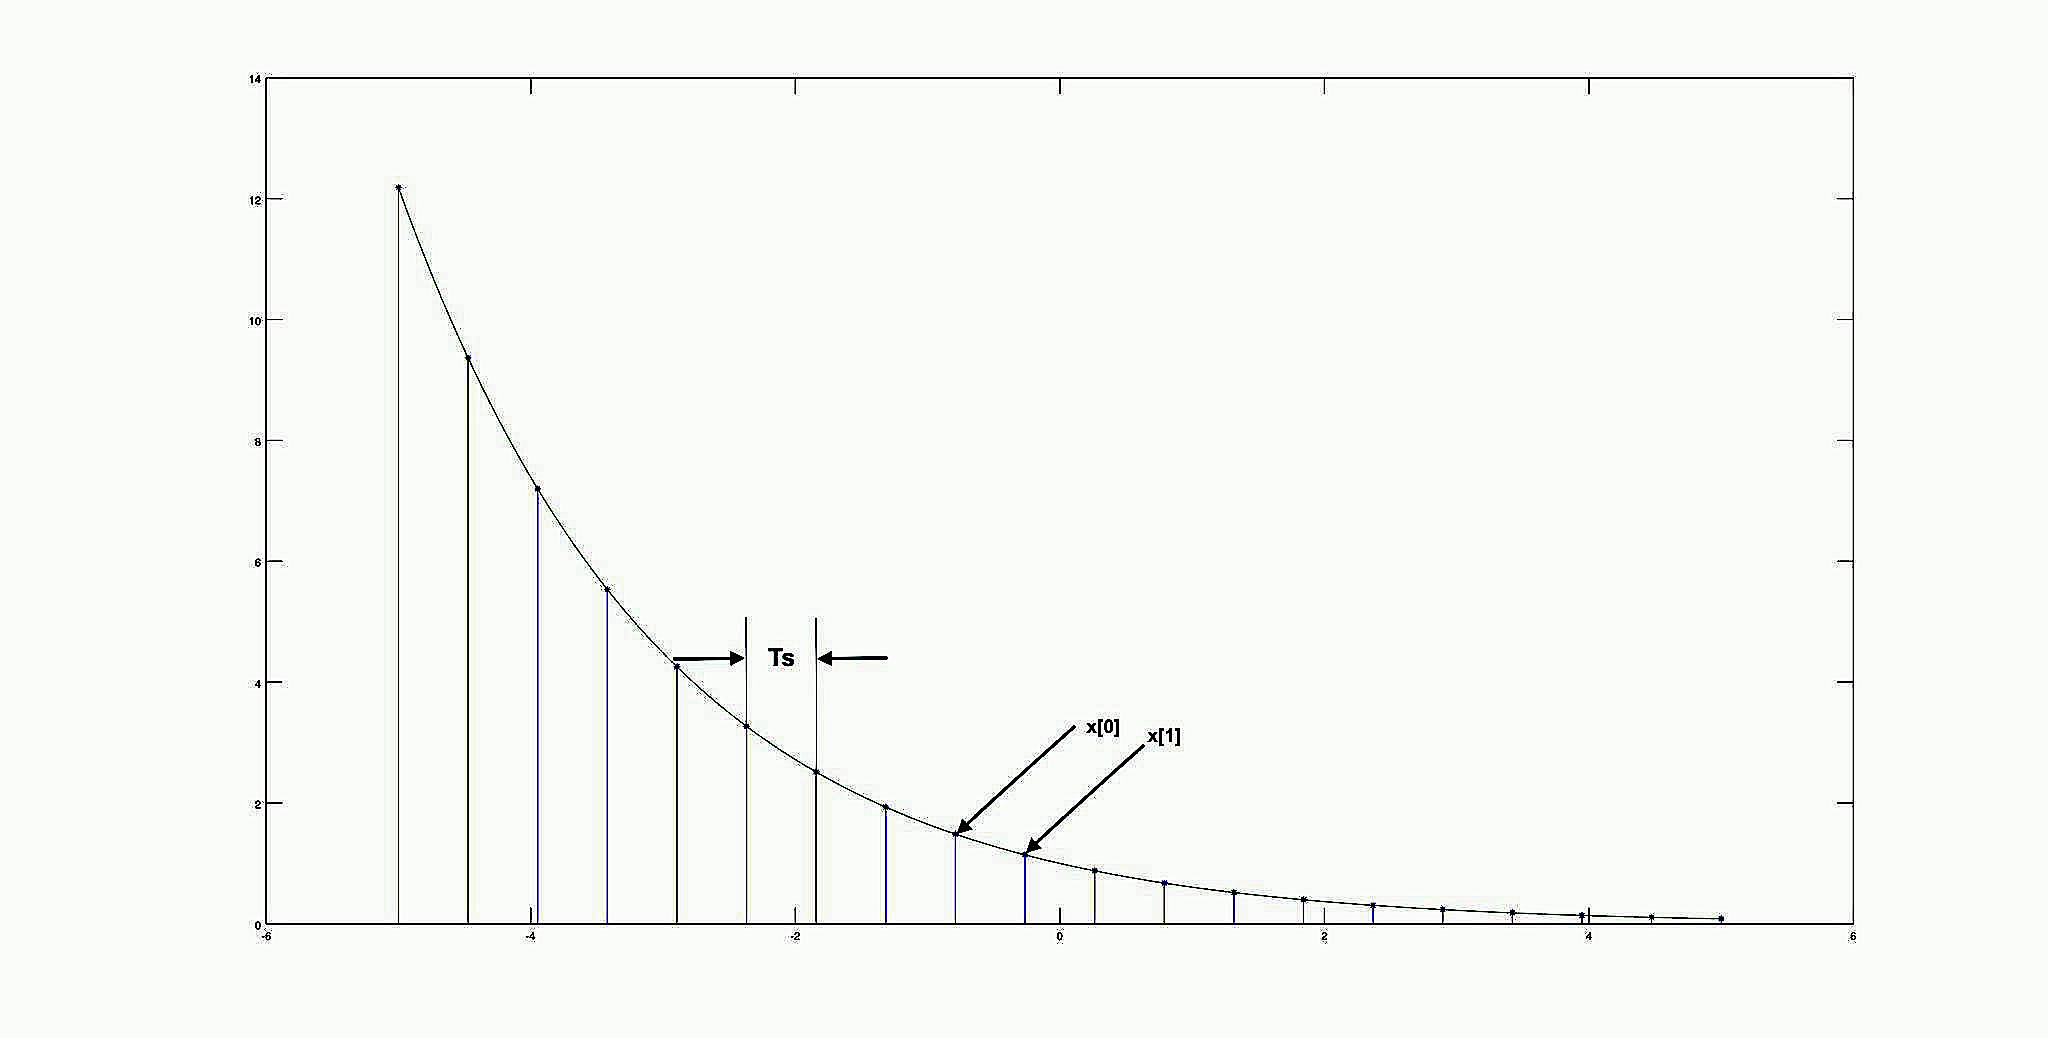
\includegraphics[width=\textwidth]{sampled.jpeg}
\end{figure}

In fig. 1, we see a continuous time signal $x(t)$ being sampled at a frequency of $1/T_{s}$ where $T_{s}$ is the length of the $sampling$ $interval$. The origin (the point $t=0$) of the resulting discrete signal can be assigned as per convenience.\\

We obtain, then, from the continuous signal, a discrete signal which, in some ways, is similar to the orignal continuous signal; it is a replica of the continuous signal. Music lovers might be like, ``Wait a minute! Aren't we loosing out on a lot of information in doing that? Won't my music sound bad?" We, however, resort to some clever techniques so that this loss is not perceptible to the human senses. And we can always resort to a higher sampling frequency. Thus, in the case of an audio CD, the sampling rate is 44,100 Hz i.e. we sample the audio signal 44,100 times in a second! We hope, thus, that we do not loose out a lot on the human experience of the music (or the image or video. Yes even the images we deal with these days are discretised. In what way do you think is this done?).\\

In this module, we set out to answer this basic about sampling a continuous time signal. We recognise that it is necessary and convenient to sample the signal as mentioned above. However,we must ask ourselves if the sampling we perform is even meaningful; meaningful in the sense that this sampling does not cost us a lot. We might loose information when sampling. Is this information loss tolerable or can we process the signals (both the sampled and the orignal) so that the result is acceptable. Or should we just increase the sampling frequency? While pondering over these, we must remember the enormous benefits sampling provides us. Thus it is a trade off and we would attempt to provide an analytical approach to solve this dilemma in the future lectures. While studying this, we explore the aforementioned connection between discrete and continuous signals and systems.

\subsection{A Priori Information}
When going from a continuous signal to a sampled version of it, we noted above that we might end up loosing some information contained in the orignal signal i.e. the signal reconstructed from the sampled signal may not resemble the orignal signal as much as we might want it to. The central idea in determining if this is the case, if reconstructing the original signal is simple or hard is the idea of apriori information. Apriori information is the information we have about the signal before we start the process of reconstruction. We illustrate this idea with a series of examples below.\\

\subsubsection{Some Examples}
\subsubsection{Some Easy Cases}
Consider a constant continuous signal $x(t) = \alpha, \alpha \in \mathbb{R}$. We ask the question in the context of this signal now. Can we sample and reconstruct this signal? If so, how do we go about doing this? If we have the a priori information that the signal is a constant signal, then we just need to know the value of $\alpha$ to have complete knowledge about the signal so that we can reconstruct it fully. This can be achieved by sampling the signal at just one value of $t$, say $t_{0}$. As $x(t_{0}) = \alpha$ we get the value of $\alpha$ as required.\\

Consider now the situation where we know beforehand that the signal under consideration is zero everywhere. Then, in order to reconstruct it, we need no samples at all. Even in the case of a non trivial signal like a sinusoid given by $x(t) =  5cos(4t+2)$, if know that the signal is $x(t) = 5cos(4t+2)$, we do not need any samples to reconstruct the signal.\\

These examples bring out an important idea. The more a priori information we have, the less is the amount of effort needed to sample and reconstruct the signal. 

\subsubsection{Reconstructing an Exponential Signal}
Consider the case where the a priori information we have is that the signal is an exponential signal. Thus the signal is of the form $x(t) = A_{0}e^{\alpha t}$. In order to sample and reconstruct this signal, we observe that we need two samples, say at times $t_{1}$ and $t_{2}$. The values of the samples will thus be $x(t_{1})$ and $x(t_{2})$ respectively. Then, we obtain the following two equations.
\begin{equation}
    x(t_{1}) = A_{0}e^{\alpha t_{1}}
\end{equation}

\begin{equation}
    x(t_{2}) = A_{0}e^{\alpha t_{2}}
\end{equation}

Dividing the $(1)$ by $(2)$ and taking the natural logarithm on both sides, we obtain
\[
    \alpha = \frac{ln(x(t_{2})) - ln(x(t_{1}))}{t_{2}-t_{1}}
\]

Substituting this value of $\alpha$ in $(1)$, we obtain,
\[
    A_{0} = x(t_{1})e^{-\alpha t_{1}}
\]

Thus, samples at two finite times enable us to reconstruct the signal entirely with the a priori infirmation we have.

\subsubsection{Making the Problem Harder: A Sum of Exponentials}
Suppose we just know that the signal is finite sum of exponentials. Thus, if $M \in \mathbb{Z}$, 

\[
    x(t) = A_{1}e^{\alpha_{1} t} + A_{2}e^{\alpha_{2} t} + ... + A_{M}e^{\alpha_{M} t}
\]

If $M$ is unknown too, this problem is very hard to solve. Thus, for the purposes of illustration, we assume that $M$ is known. In that case, we have $2M$ unknowns, $\alpha_{1}$, $\alpha_{2}$, ...,$\alpha_{M}$ and $A_{1}$, $A_{2}$, ..., $A_{M}$. Thus, we need $2M$ samples to be able to reconstruct the signal entirely. Let the samples be taken at times $t_{1}$, $t_{2}$, ..., $t_{2M}$. In this case, we get the following system of equations,
\begin{align*}
    A_{1}e^{\alpha_{1} t_{1}} + A_{2}e^{\alpha_{2} t_{1}} + ... + A_{M}e^{\alpha_{M} t_{1}} &= x(t_{1})\\
    A_{1}e^{\alpha_{1} t_{2}} + A_{2}e^{\alpha_{2} t_{2}} + ... + A_{M}e^{\alpha_{M} t_{2}} &= x(t_{2})\\
.\\.\\.\\
    A_{1}e^{\alpha_{1} t_{2M}} + A_{2}e^{\alpha_{2} t_{2M}} + ... + A_{M}e^{\alpha_{M} t_{2M}} &= x(t_{2M})\\
\end{align*}

As can be seen however, this system of equations is highly non-linear in the unknowns and hence it is not exactly clear how a solution might be obtained. At this stage, we simplify the problem further. We assume that $\alpha_{1}$, $\alpha_{2}$, ...,$\alpha_{M}$ are known. In this case, $M$ samples suffice and we get the following system of equations.

\begin{align*}
    A_{1}e^{\alpha_{1} t_{1}} + A_{2}e^{\alpha_{2} t_{1}} + ... + A_{M}e^{\alpha_{M} t_{1}} &= x(t_{1})\\
    A_{1}e^{\alpha_{1} t_{2}} + A_{2}e^{\alpha_{2} t_{2}} + ... + A_{M}e^{\alpha_{M} t_{2}} &= x(t_{2})\\
.\\.\\.\\
    A_{1}e^{\alpha_{1} t_{M}} + A_{2}e^{\alpha_{2} t_{M}} + ... + A_{M}e^{\alpha_{M} t_{M}} &= x(t_{M})\\
\end{align*}

Then, this is a system of linear equations in $A_{1}$, $A_{2}$, ..., $A_{M}$. The fact that this systems is obtained by sampling a sum of exponentials guarantees that the $M$ equations are all independent and that a solution exists. This solution is also easily computable.\\

One can also assume, however, that the $A_{1}$, $A_{2}$, ..., $A_{M}$ are known and that $\alpha_{1}$, $\alpha_{2}$, ..., $\alpha_{M}$ are unknowns. We get the same system of equations as in the previous case. How can one solve this system to obtain $\alpha_{1}$, $\alpha_{2}$, ..., $\alpha_{M}$? We leave this as an exercise to the students. 

